
% \documentclass[aoas,preprint]{imsart}
\documentclass[preprint]{imsart}

\RequirePackage[OT1]{fontenc}
\RequirePackage{amsthm,amsmath}
\RequirePackage[numbers]{natbib}
\RequirePackage[colorlinks,citecolor=blue,urlcolor=blue]{hyperref}


\usepackage{amsmath,amsthm,amsfonts}
\usepackage{changepage}
\usepackage{amssymb}
\usepackage{graphicx}%
\usepackage{color}
\usepackage{float}
\usepackage{epstopdf}
\usepackage{graphicx}
\usepackage{subcaption}
\usepackage[ruled, vlined]{algorithm2e}


% settings
%\pubyear{2005}
%\volume{0}
%\issue{0}
%\firstpage{1}
%\lastpage{8}
% \arxiv{arXiv:0000.0000}

\startlocaldefs
\numberwithin{equation}{section}
\theoremstyle{plain}
\newtheorem{thm}{Theorem}[section]
% This is the file with definitions

%%%%%%%%%%%%%%%%%%%%%%%%%%%%%%%%%%%%%%%%%%%%%

\newcommand{\complexunit}{\text{i}}

\newcommand{\be}{\begin{equation}}
\newcommand{\ee}{\end{equation}}
\newcommand{\bes}{\begin{equation*}}
\newcommand{\ees}{\end{equation*}}
\newcommand{\beqn}{\begin{eqnarray}}
\newcommand{\eeqn}{\end{eqnarray}}
\newcommand{\beqns}{\begin{eqnarray*}}
\newcommand{\eeqns}{\end{eqnarray*}}
\newcommand{\bea}{\begin{align}}
\newcommand{\eea}{\end{align}}
\newcommand{\beas}{\begin{align*}}
\newcommand{\eeas}{\end{align*}}


\newcommand{\lkr}{\left(}
\newcommand{\lkv}{\left[}
\newcommand{\rkv}{\right]}
\newcommand{\rkr}{\right)}
\newcommand{\lfi}{\left\{}
\newcommand{\rfi}{\right\}}

\newcommand{\fr}[1]{(\ref{#1})}

\newcommand{\vart}{\vartheta}
\newcommand{\ro}{\varrho}
\newcommand{\ph}{\varphi}
\newcommand{\del}{\delta}
\newcommand{\Del}{\Delta}
\newcommand{\dn}{\delta_n}
\newcommand{\al}{\alpha}
\newcommand{\af}{\alpha}
%\newcommand{\eps}{\varepsilon}
\newcommand{\eps}{\epsilon}
\newcommand{\Ga}{\Gamma}
\newcommand{\ga}{\gamma}
\newcommand{\te}{\theta}
\newcommand{\om}{\omega}
\newcommand{\lam}{\lambda}
\newcommand{\Up}{\Upsilon}
\newcommand{\up}{\upsilon}
\newcommand{\dz}{\zeta}
\newcommand{\sig}{\sigma}
\newcommand{\sgmd}{\sigma^2}
\newcommand{\Lam}{\Lambda}
\newcommand{\Om}{\Omega}
\newcommand{\Sig}{\Sigma}


\newcommand{\EE}{\ensuremath{{\mathbb E}}}
\newcommand{\JJ}{\ensuremath{{\mathbb J}}}
\newcommand{\II}{\ensuremath{{\mathbb I}}}
\newcommand{\ZZ}{\ensuremath{{\mathbb Z}}}
\newcommand{\PP}{\ensuremath{{\mathbb P}}}
\newcommand{\QQ}{\ensuremath{{\mathbb Q}}}
\newcommand{\KK}{\ensuremath{{\mathbb K}}}
\newcommand{\RR}{\ensuremath{{\mathbb R}}}


\newcommand{\low}{\mbox{low}}
\newcommand{\vect}{\mbox{vec}}
\newcommand{\Pen}{\mbox{Pen}}
\newcommand{\Span}{\mbox{Span}}
\newcommand{\intg}{\mbox{int}}
\newcommand{\card}{\mbox{card}}
\newcommand{\Range}{\mbox{Range}}
\newcommand{\Var}{\mbox{Var}}
\newcommand{\Cov}{\mbox{Cov}}
\newcommand{\diag}{\mbox{diag}}
\newcommand{\supp}{\mbox{supp}}
\newcommand{\etal}{{\it et  al. }}
\newcommand{\std}{\mbox{std}}
\newcommand{\SNR}{\mbox{SNR}}
\newcommand{\Tr}{\mbox{Tr}}
\newcommand{\proj}{\mbox{proj}}
\newcommand{\bal}{\mbox{\small bal}}
 


\newtheorem{theorem}{Theorem}
\newtheorem{lemma}{Lemma}
\newtheorem{corollary}{Corollary}
\newtheorem{proposition}{Proposition}
\newtheorem{assumption}{Assumption}
\newtheorem{remark}{Remark}
\newtheorem{example}{Example}
\newtheorem{definition}{Definition}


\newcommand{\ba}{\mathbf{a}}
\newcommand{\bb}{\mathbf{b}}
\newcommand{\bc}{\mathbf{c}}
\newcommand{\bd}{\mathbf{d}}
\newcommand{\boe}{\mathbf{e}}
\newcommand{\bof}{\mathbf{f}}
\newcommand{\bg}{\mathbf{g}}
\newcommand{\bi}{\mathbf{i}}
\newcommand{\bj}{\mathbf{j}}
\newcommand{\bk}{\mathbf{k}}
\newcommand{\bh}{\mathbf{h}}
\newcommand{\bq}{\mathbf{q}}
\newcommand{\bt}{\mathbf{t}}
\newcommand{\bu}{\mathbf{u}}
\newcommand{\bv}{\mathbf{v}}
\newcommand{\bw}{\mathbf{w}}
\newcommand{\bx}{\mathbf{x}}
\newcommand{\by}{\mathbf{y}}
\newcommand{\bz}{\mathbf{z}}

\newcommand{\bA}{\mathbf{A}}
\newcommand{\bB}{\mathbf{B}}
\newcommand{\bC}{\mathbf{C}}
\newcommand{\bD}{\mathbf{D}}
\newcommand{\bF}{\mathbf{F}}
\newcommand{\bG}{\mathbf{G}}
\newcommand{\bI}{\mathbf{I}}
\newcommand{\bH}{\mathbf{H}}
\newcommand{\bM}{\mathbf{M}}
\newcommand{\bQ}{\mathbf{Q}}
\newcommand{\bS}{\mathbf{S}}
\newcommand{\bU}{\mathbf{U}}
\newcommand{\bV}{\mathbf{V}}
\newcommand{\bW}{\mathbf{W}}
\newcommand{\bX}{\mathbf{X}}
\newcommand{\bY}{\mathbf{Y}}
\newcommand{\bZ}{\mathbf{Z}}

\newcommand{\bzero}{\mathbf{0}}
\newcommand{\bone}{\mathbf{1}}


 \newcommand{\blam}{\mbox{\mathversion{bold}$\lam$}}
 \newcommand{\bte}{\mbox{\mathversion{bold}$\te$}}
\newcommand{\bxi}{\mbox{\mathversion{bold}$\xi$}}
\newcommand{\boeta}{\mbox{\mathversion{bold}$\eta$}}
\newcommand{\bbe}{\mbox{\mathversion{bold}$\beta$}}
\newcommand{\bzeta}{\mbox{\mathversion{bold}$\zeta$}}
\newcommand{\bph}{\mbox{\mathversion{bold}$\ph$}}
\newcommand{\bpsi}{\mbox{\mathversion{bold}$\psi$}}
\newcommand{\beps}{\mbox{\mathversion{bold}$\eps$}}
\newcommand{\bobeta}{\mbox{\mathversion{bold}$\beta$}}
\newcommand{\bgamma}{\mbox{\mathversion{bold}$\gamma$}}
\newcommand{\bom}{\mbox{\mathversion{bold}$\om$}}

\newcommand{\bbJ}{(\bb_J)}

\newcommand{\bPhi}{\mbox{\mathversion{bold}$\Phi$}}
\newcommand{\bUp}{\mbox{\mathversion{bold}$\Up$}}
\newcommand{\bPsi}{\mbox{\mathversion{bold}$\Psi$}}
\newcommand{\bLam}{\mbox{\mathversion{bold}$\Lambda$}}
\newcommand{\bSig}{\mbox{\mathversion{bold}$\Sigma$}}
\newcommand{\bTe}{\mbox{\mathversion{bold}$\Theta$}}
\newcommand{\bXi}{\mbox{\mathversion{bold}$\Xi$}}
\newcommand{\bPi}{\mbox{\mathversion{bold}$\Pi$}}


\newcommand{\Jc}{{J^c}}

\newcommand{\calB}{{\mathcal{B}}}
\newcommand{\calC}{{\mathcal{C}}}
\newcommand{\calD}{{\mathcal{D}}}
\newcommand{\calF}{{\mathcal{F}}}
\newcommand{\calG}{{\mathcal G}}
\newcommand{\calH}{{\cal H}}
\newcommand{\calJ}{{\mathcal{J}}}
\newcommand{\calK}{{\mathcal{K}}}
\newcommand{\calL}{{\mathcal{L}}}
\newcommand{\calM}{{\mathcal M}}
\newcommand{\calN}{{\cal N}}
\newcommand{\calP}{{\mathcal{P}}}
\newcommand{\calS}{{\mathcal{S}}}
\newcommand{\calT}{{\cal T}}
\newcommand{\calW}{{\cal W}}
\newcommand{\calX}{{\cal{X}}}
\newcommand{\calY}{{\cal{Y}}}
\newcommand{\calZ}{{\cal{Z}}}
 
 
\newcommand{\lan}{\langle}
\newcommand{\ran}{\rangle}
 
 
%%%%%%%%%%%%%%%%%%%%%%%%%%%%%%%%%%%%%%%%%%%%%%%%%%%%%%%%%%%%%%%%%%%%%%%%%%%%%%%%%%%%%

\newcommand{\sumjp}{\sum_{j=1}^p}
\newcommand{\sumin}{\sum_{i=1}^n}
\newcommand{\sumJ}{\sum_{j \in J}}
\newcommand{\sumJc}{\sum_{j \in \Jc}}


\newcommand{\hbLam}{\widehat{\bLam}} 
\newcommand{\hbd}{\widehat{\bd}}
\newcommand{\hbC}{\widehat{\bC}}
\newcommand{\hbS}{\widehat{\bS}}
\newcommand{\hbq}{\widehat{\bq}}
\newcommand{\hbte}{\widehat{\bte}}
\newcommand{\hbTe}{\widehat{\bTe}}
\newcommand{\hbW}{\widehat{\bW}}
\newcommand{\hbV}{\widehat{\bV}}
\newcommand{\hbZ}{\widehat{\bZ}}
\newcommand{\hbUp}{\widehat{\bUp}}
\newcommand{\hbUphJ}{\hbUp_{\hbC,\hJ}}
\newcommand{\hbPi}{\widehat{\bPi}}


\newcommand{\tilbC}{\tilde{\bC}}
\newcommand{\tilbF}{\tilde{\bF}}
\newcommand{\tilbZ}{\tilde{\bZ}}
\newcommand{\tilbq}{\tilde{\bq}}
 

\newcommand{\hm}{\widehat{m}}
\newcommand{\hJ}{\widehat{J}}
\newcommand{\hM}{\widehat{M}}
\newcommand{\hrho}{\widehat{\rho}}


\newcommand{\bds}{{\bd^*}}
\newcommand{\bDs}{\bD^*}
\newcommand{\bQs}{{\bQ^*}}
\newcommand{\bCs}{{\bC^*}}
\newcommand{\bqs}{{\bq^*}}
\newcommand{\btes}{{\bte^*}}
\newcommand{\bLams}{{\bLam^*}}
\newcommand{\bWs}{{\bW^*}}
\newcommand{\bPhis}{{\bPhi^*}}
\newcommand{\bTes}{{\bTe^*}}
\newcommand{\bSs}{{\bS^*}}



\newcommand{\ms}{{m^*}}
\newcommand{\Js}{{J^*}}
\newcommand{\Ms}{{M^*}}%{{\ms(\ms+1)/2}}
\newcommand{\tilS}{\tilde{S}}
\newcommand{\calKsMs}{\calK^{*}_{\Ms}}
\newcommand{\Mos}{M^{*}_0}


% \newcommand{\PJ}{\bPi_J}
% \newcommand{\PJo}{\bPi_J^{\bot}}
% \newcommand{\PhJ}{\bPi_{\hJ}}
% \newcommand{\hPhJ}{\widehat{\bPi}_{\hJ}}
% \newcommand{\hPhJo}{\widehat{\bPi}_{\hJ}^{\bot}}


\newcommand{\PJ}{\bPi_{\bC,J}}
\newcommand{\PJo}{\bPi_{\bC,J}^{\bot}}
\newcommand{\PhJ}{\bPi_{\hJ}}
\newcommand{\hPhJ}{\widehat{\bPi}_{\hbC,\hJ}}
\newcommand{\hPhJo}{\widehat{\bPi}_{\hbC,\hJ}^{\bot}}




\newcommand{\PCJ}{\bPi_{\bC,J}}
\newcommand{\PCJs}{\bPi_{\bCs,J}}
\newcommand{\PCJso}{\bPi^{\bot}_{\bC^*,J}}
\newcommand{\PCJo}{\bPi_{\bC,J}^{\bot}}
\newcommand{\hPChJ}{\widehat{\bPi}_{\hbC,\hJ}}
\newcommand{\hPChJo}{\widehat{\bPi}_{\hbC,\hJ}^{\bot}}


\newcommand{\PSJ}{\bPi_{\bS,J}}
\newcommand{\PSJo}{\bPi_{\bS,J}^{\bot}}
\newcommand{\hPShJ}{\widehat{\bPi}_{\hbS,\hJ}}
\newcommand{\hPShJo}{\widehat{\bPi}_{\hbS,\hJ}^{\bot}}

\newcommand{\rhons}{\rho_n^{*}}


\newcommand{\bPhiJ}{\bPhi_J}
\newcommand{\bPhihJ}{\bPhi_{\hJ}}

 
\newcommand{\phj}{\ph_j}
\newcommand{\psij}{\psi_j}

\newcommand{\CDel}{C_{\Del}}

\newcommand{\bl}{b_l}
\newcommand{\blo}{b_{l+1}}
\newcommand{\gl}{g_l}
\newcommand{\glo}{g_{l+1}}

\newcommand{\tCo}{\tilde{C}_0}
 
%%%%%%%%%%%%%%%%%%%%%%%%%%%%%%%%%%%%%%%%%%%%%%%%%%%%%%%%%%%%%%%%%%%%%%%%%%%%%%%%%%%%%


\newcommand {\colred}[1] {\textcolor{red}{#1}}
\newcommand {\colblue}[1] {\textcolor{blue}{#1}}
\newcommand {\colyellow}[1] {\textcolor{yellow}{#1}}
\newcommand {\colblack}[1] {\textcolor{black}{#1}}
\newcommand {\colgreen}[1] {\textcolor{OliveGreen}{#1}}
\newcommand {\colsred}[1] {\textcolor{OrangeRed}{#1}}
 
%%%%%%%%%%%%%%%%%%%%%%%%%%%%%%%%%%%%%%%%%%%%%%%%%%%%%%%%%%%%%%%%%%%%%%%%%%%%%%%%%%%%%

\long\def\ignore#1{}

%%%%%%%%%%%%%%%%%%%%%%%%%%%%%%%%%%%%%%%%%%%%%%%%%%%%%%%%%%%%%%%%%%%%%%%%%%%%%%%%%%%%%

\endlocaldefs

\begin{document}

\begin{frontmatter}
\title{Understanding  developing networks with stochastic block models\thanksref{T1}}
\runtitle{Understanding  developing networks}
\thankstext{T1}{Footnote to the title with the ``thankstext'' command.}

\begin{aug}
\author{\fnms{Zitong} \snm{Zhang}\thanksref{t1,t2,m1}\ead[label=e1]{zztzhang@ucdavis.edu}},
\author{\fnms{Shizhe} \snm{Chen}\thanksref{t3,m1}\ead[label=e2]{szdchen@ucdavis.edu}}
% \and
% \author{\fnms{Third} \snm{Author}\thanksref{t1,m1}
% \ead[label=e3]{third@somewhere.com}
% \ead[label=u1,url]{http://www.foo.com}}

\thankstext{t1}{Some comment}
\thankstext{t2}{First supporter of the project}
\thankstext{t3}{Second supporter of the project}
\runauthor{Z. Zhang and S. Chen}

\affiliation{University of California Davis\thanksmark{m1}}

\address{Address of the First and Second authors\\
Usually a few lines long\\
\printead{e1}\\
% \phantom{E-mail:\ }\printead*{e2}
}

% \address{Address of the Third author\\
% Usually a few lines long\\
% Usually a few lines long\\
% \printead{e3}\\
% \printead{u1}}
\end{aug}


%!TEX root = Main.tex

\begin{abstract}
 In neuroscience, it is not well understood how newborn neurons form a mature nervous system, due to the lack of observations. A recent study (Wan et al. 2019) made available a dataset of this functional maturation process on zebrafish. This novel data, however, introduce inherent challenges for the analysis of the formation of the nervous system.  First, the formation process is transient by nature.  The non-stationarity of the process makes the amount of data pale in comparison to the size of the neural network.  Moreover, combining observations on multiple subjects are not straightforward since the neural circuits are not identical across subjects.   In this talk, we propose a model for describing the emergence of a coordinated network from isolated nodes.  To this end, we adapt and generalize the stochastic block model for random graphs. The proposed method learns the transferable features across subjects, while allowing for individual variabilities. Briefly, the proposed method classifies nodes into different functional groups by identifying typical connecting behavior. We further employ the shape invariant models to handle the nodal delays due to neuron-specific delays.  We establish the consistency and minimax optimality of the proposed estimator.  We demonstrate the performance of our algorithm on simulation experiments, and on the real zebrafish dataset.
\end{abstract}



\begin{keyword}[class=MSC]
\kwd[Primary ]{60K35}
\kwd{60K35}
\kwd[; secondary ]{60K35}
\end{keyword}

\begin{keyword}
\kwd{sample}
\kwd{\LaTeXe}
\end{keyword}

\end{frontmatter}



%!TEX root = Main.tex


\section{Introduction}

% \subsection*{Motivation}
Dynamic networks emerge in many area,
such as the neuronal network in the brain during disease[] or learning tasks[], 
the social network in a time period[], etc.
A lot of work has been done in order to study the dynamic networks,
but most of these research focus on analyzing the dynamics in a well-developed network.
In this paper, we concentrate on the growing networks where a bunch of isolated nodes are developed into a functional network.
To the best of our knowledge, there is no existing study about the growing networks, partly because of the lack of data.
Fortunately, the data collected by \citet{Wan2019} provides us the possibility to pursue this study.


Since a functional network is complicated, we try to break it down and propose to model it by identifying the typical roles of individual nodes. 
As supported by \cite{Wan2019}, neurons in a patterned network have different roles in terms of active time and connecting patterns. 
The connecting pattern of a neuron can be described as a collection of point processes representing the connection between this neuron and each of the rest individual neurons.
Neurons with the same roles perform similar activities and thus have similar connecting patterns. 



However, being able to identify the typical roles in a single growing network is not satisfactory because 
the growing network data is transient --- there is only one measurement for each subject, which means we only have one sample for estimation.
Also, the roles identified from different subjects are not comparable, because the neurons and the networks are not one-to-one mapped. 
This constrains our ability to study the common features across subjects.
For this reason, we propose to use the stochastic block model as it allows to combine multiple networks and hence resolve the above problems.


There are, nevertheless, some unique properties of the data that are beyond the scope of the stochastic block model.
First, the connection between two neurons is measured over time.
Second, the connecting pattern between two neurons are determined not only by their roles but also by their active time, which varies from node to node.
Third, the connection is also effected by the spatial distance between neurons --- connection cannot occur if two neurons are too away from each other.
To incorporate such uniqueness, we propose a generalized stochastic block model in this paper.


\subsection*{Related work}
	The stochastic block model is first proposed by \citet{Holland1983}.
	It has many dynamic extensions,
	\citet{Yang2011,Xu2014a,Matias2016,Xu2015} use the Markov chain to model the time-varying  connecting probabilities and/or the clustering matrix. 
	EM algorithm or iterative optimization algorithm is commonly used for inference.

	 \citet{Matias2018} adapt the stochastic block model to the context of recurrent interaction events in continuous time, 
	where the recurrent events are modeled by Poisson processes with intensities determined by the nodes' group memberships. 
	The maximum likelihood estimator is proposed, but no theoretical analysis is available in the paper. 

	Optimal rate of convergence is also studied.
	\citet{Gao2015a} provides an optimal rate under the mean squared error for the stochastic block model.
	\citet{Pensky2019a} 
	% proposes a vectorization technique to simplify the tensor estimation in the dynamic network setting, and 
	derives a penalized least square estimator in a dynamic network setting, and shows that the estimator satisfies an oracle inequality and  attains the minimax lower bound for the risk.


	% \item Convex relaxation methods for community detection have been studied in \citet{Li2018,Li2017,Peng2005}.



\subsection*{Contribution}
	In this paper, we propose a method for analyzing the growing networks. Our method is able to identify the roles of individual nodes and the connecting patterns.
	We adapt the stochastic block model to the growing networks context by generalizing the connecting probabilities to intensities of point processes. 
	In addition, we incorporate the time delay of each node so that our model is able to handle the network where nodes become active over time.
	We derive a least square estimator and show that the estimator converges [in a certain rate].
	Finally, an algorithm combining the k-means method and the shape invariant method is proposed for estimation.



\subsection*{Future work}
Future working directions include (but not limited to)
	(i) identifying clusters with similar connecting pattern but different active time phase or different vertex degree,
	(ii) incorporating the movement of nodes,
	(iii) seeking for a convex relaxation method that convexify over both clustering matrix and time lags
	(convex relaxation can also be adapted to solve the penalized least square problem in \citet{Pensky2019a}),
	(iv) try other clustering methods.





\subsection*{Organization}
The rest of this paper is organized as follows. 
In Section \ref{sec:model}, we review the stochastic block model and introduce the proposed dynamic generalization of the stochastic block model.
We introduce the least square estimator and the estimation algorithm in Section \ref{sec:method}.
Theoretical results are provided in Section \ref{sec:theory}. Section \ref{sec:simulation} shows the numerical experiments.






%!TEX root = Main.tex

\section{Model} %%% introcude $Gamma_a, a=1,\cdots,k$ somewhere in this section!
% \subsection{Notations}


\subsection{Stochastic block model} % deleted the "undirected" setting
A set of $n$ nodes $\Gamma=\left\{ v_1,\cdots,v_n \right\}$ is partitioned into $k$ clusters $\Gamma_1,\cdots,\Gamma_k$. For simplicity, we use the notation $i\in\Gamma_l$ to denote that $v_i\in\Gamma_l$. The cluster of node $v_i$ is represented by $z_i\in \left\{ 1,\cdots,k \right\}$, and the vector of clusters is $\bz=\left( z_i \right)_{i=1}^n $. 
Define the adjacency matrix $\bA\in \left\{ 0,1\right\}^{n\times n}$ where  $\bA_{i,j}= 1$ if an edge is observed between $v_i$ and $v_j$ and $\bA_{i,j}=0$ otherwise.
We set $\mathbf{A}_{i,i}\equiv 0$  for any $i=1,\cdots,n$, 
and assume that $\bA_{i,j}$'s are conditionally independent given the cluster vector $\bz$:
\begin{align*}
\mathbf{A}_{i,j}|z_i=q,z_j=l \overset{ind}{\sim} \text{Bernoulli}(\mathbf{C}_{q,l}), \qquad i\neq j,
\end{align*}
where $\mathbf{C}\in [0,1]^{k\times k}$ denote the  connecting probability matrix.



\subsection{Dynamic generalization of the stochastic block model}
Consider a growing dynamic network where edges appear over time. 
Assume that the edges will not disappear once constructed,
and that the observed point processes ${N}_{i,j}(\cdot)\in \left\{ 0,1 \right\}$ are independent realizations of intensity functions 
\begin{align*}
\lambda_{i,j}(t)=f_{z_i,z_j}(t-\tau_{i,j})\cdot g(d_{i,j}), \qquad t\in[0,T],\quad i,j=1,\cdots,n, 
\end{align*}
where $[0,T]$ is overall time period,
$\tau_{i,j}$ is the time lag of the edge from $v_i$ to $v_j$, 
 $d_{i,j}$ is the spatial distance between $v_i$ and $v_j$, $f_{z_i,z_j}(\cdot)$ is the connecting intensity function from cluster $z_i$ to $z_j$, and $g(\cdot)$ is a decreasing function that accounts for the decay of connection as the distance between any pair of nodes increases.
Similar to the stochastic block model, we set $\lambda_{i,i}(\cdot)\equiv 0$ for $i=1,\cdots,n$.
% Add more rigorous definition of point process and intensity function.
\\
The integrated point process $N_{i,\cdot}(\cdot):=\sum_{j\neq i} N_{i,j}(\cdot)$ can be viewed as a realization of the intensity function $\lambda_{i,\cdot}(\cdot)=\sum_{j\neq i}\lambda_{i,j}(\cdot)$.
For convenience, we denote $N_{i,\cdot}(\cdot)$ by $N_i(\cdot)$, and $\lambda_{i,\cdot}(\cdot)$ by $\lambda_{N_i}(\cdot)$. 

In many applications, the edge from $v_i$ to $v_j$ is determined only by the activity of $v_i$. 
So we may have the following assumption.
\begin{assumption}\label{asp:time lag}
$\tau_{i,j}$ only depends on $v_i$, that is,
$\tau_{i,j}=\tau_i $ for all $j\neq i, i=1,\cdots,n$.
\end{assumption}
\noindent With Assumption \ref{asp:time lag}, $\lambda_{N_i}(\cdot)$ can be written as
\begin{align*}
\lambda_{N_i}(t) &= \sum_{l=1}^k \left( f_{z_i,l}(t-\tau_i)\cdot \sum_{j\in\Gamma_l,j\neq i}g(d_{i,j}) \right) \\
&=: \sum_{l=1}^k  f_{z_i,l}(t-\tau_i)\cdot w_{i,l}.
\end{align*}
Here $w_{i,l}$ measures the overall distance between node $v_i$ and cluster $\Gamma_l$. 
For example, if the nodes represent neurons and are clustered by cell types, $w_{i,l}$ represents the distance between $v_i$ and its neighbor cells  which belong to cell types $l$.
We assume that the cell types are distributed uniformly in the sense that $w_{i,l}$ and $w_{j,l}$ are identically distributed for any $i, j$ such that $z_i=z_j$.
More formally, we have the following assumption.
 % which means $w_{i,l}=\bar w_{z_i,l}+\epsilon_{i,l}$ where $\left\{ \epsilon_{i,l} \right\}_{i\in\Gamma_l}$ are i.i.d. random variables with mean zero.

\begin{assumption}\label{asp:same distr}
$w_{i,l}=\bar w_{z_i,l}+\epsilon_{i,l}$ where $\left\{ \epsilon_{i,l} \right\}_{i\in\Gamma_l,l=1,\cdots,k}$ are i.i.d. random variables with mean $0$ and variance $\sigma^2<\infty$.
\end{assumption}
\noindent
By Assumption \ref{asp:time lag} and \ref{asp:same distr}, $\lambda_{N_i}(t)=\lambda_{z_i}(t-\tau_i)+\sum_{l=1}^kf_{z_i,l}(t-\tau_i)\epsilon_{i,l}$ for $t\in[0,T]$, where $\lambda_{z_i}(t):=\sum_{k=1}^lf_{z_i,l}(t)\cdot\bar w_{z_i,l}$.

\subsubsection*{Minor comments}
Hoeffding's inequality might be useful later. (If $\epsilon_{1},\cdots,\epsilon_d\overset{i.i.d}{\sim}\text{sub-G}(\tau_0)$ and $\mathbb{E}\epsilon_{i}=0$, then $\mathbb{P}(\langle a,\epsilon\rangle\geq t)\leq \exp \left\{ -t^2/(2\|a\|_2^2\tau_0^2) \right\}$ for any $a\in \mathbb{R}^d$.)

Let $\mathbf{F}_{k\times k} = [f_{q,l}(\cdot)]_{q,l\in \left\{ 1,\cdots,k \right\}}$, $\mathbf W_{n\times k} = [w_{i,l}]_{i\in \left\{ 1,\cdots,n \right\}, l\in \left\{ 1,\cdots,k \right\}}$, $\mathbf{Z}\in \left\{ 0,1 \right\}^{n\times k}$ with $\mathbf Z_{i,l}=1$ if $z_i=l$ and $0$ otherwise. Then
\begin{align*}
\begin{bmatrix}
\lambda_{N_1}(\cdot+\tau_1)\\
\vdots\\
\lambda_{N_n}(\cdot+\tau_n)
\end{bmatrix}=\text{diag}\left( \mathbf{ZFW}^\top \right) .
\end{align*}



%!TEX root = Main.tex


\section{Method}




	\subsection{k-means objective function}
		We will introduce the objective function of k-means in the Euclidean space as well as in our case where the samples are realizations of point process.
		\subsubsection*{k-means in $\mathbb{R}^d$} 
			Let ${\mathbf{x}_1,\cdots,\mathbf{x}_n}\in \mathbb{R}^d$ be an i.i.d. sample from distribution function $F$. Denote by $F_n$ the empirical distribution function. The k-means problem is to minimize 
			\begin{align*}
			W_n(A,F_n)=\int \min_{a\in A}\|\mathbf{x}_i-a\|^2  dF_n
			\end{align*}
			over all possible choices of the set $A$ containing $k$ points in $\mathbb{R}^d$.
			Denote by $\bar A = \arg\min_A W(A,F) $ the optimal population cluster centers, and $A_n = \arg\min_A W_n(A,F_n)$ the optimal sample cluster centers. \citet{Pollard1981a} showed that for a given $k$,
			\begin{align*}
			A_n\to \bar A \ \text{a.s.}
			\end{align*}
			{\color{red} What does $\bar A$ represent? If $k=2$ and $F(x)=\frac{1}{2}\Phi(x;\mu_1,\sigma_1^2)+\frac{1}{2}\Phi(x;\mu_2, \sigma_2^2)$ is a mixture Gaussian distribution, 
			and denote $X_1\sim N(\mu_1,\sigma_1^2)$, then I expect $\bar A= \left\{ a_1,a_2 \right\} $ where $a_1=\mathbb{E}[X_1 \mathbf{1}_{X_1\leq (\mu_1+\mu_2)/2}]\neq \mu_1 $ (and a similar expression for $a_2$). } 

			This problem can be reformulated as solving 
			\begin{equation}\label{eq:kmeans}
			\min_{\left\{ \Gamma_l \right\}_{l=1}^k}\frac{1}{n}\sum_{l=1}^k\sum_{i\in \mathbf{\gamma}_l} \|\mathbf{x}_i- \mathbf{c}_l\|^2,
			\end{equation}
			where $\left\{ \Gamma_l \right\}_{l=1}^k$ represent the clusters and form a partition of $\Gamma = \left\{ 1,2,\cdots,n \right\}$, $\mathbf{c}_l = \frac{1}{|\Gamma_l|}\sum_{i\in \Gamma_l}\mathbf{x}_i$ is the sample center of the $l$-th cluster. We now extend this objective function to the context of point process.
		\subsubsection*{k-means in point process}
			Denote by $d(N(\cdot), \lambda(\cdot))$ the distance between a point process and an intensity function. The problem of selecting distance function is discussed later.
			{\color{red} If we can assume that $N_i(t+\tau_i)\overset{d}{=}N_j(t+\tau_j)$ for any $i,j$ such that $z_i=z_j$,}
			the k-means problem is
			\begin{equation}\label{eq:kmeans_pp}
			\min_{\left\{ \Gamma_l \right\}_{l=1}^k} \frac{1}{n} \sum_{l=1}^k \left(\min_{\{\tau_i\}_{i\in\gamma_l},\lambda_l} \sum_{i\in\gamma_l} d(N_i(t+\tau_i), \lambda_l) \right).
			\end{equation}
			I expect the solution of (\ref{eq:kmeans_pp}) to converge, as $n\to\infty$, to the minimizer of the population version of this objective function. {\color{red}But what does that mean?}
			{\color{blue} Read more paper about consistency of k-means problem.}
		\subsubsection*{Distance between a point process and an intensity function}
			For a given Poisson process $N(\cdot)$ and an intensity function $\lambda(\cdot)$, the distance can be defined as the negative log-likelihood
			\begin{align*}
			d(N, \lambda) \equiv -l(N;\lambda) = \int_{0}^T\lambda(t)dt - \sum_{j=1}^{N(0,T]}\log \left( \lambda(t_j^{(N)}) \right) ,
			\end{align*}
			where $t_j^{(N)}$'s are the time of events of $N(\cdot)$.			
			{\color{blue} Justify why it is reasonable to use Poisson process. }
			% Also explain why this is a good measure of similarity.
	 		See \citet{Daley} for details.

			The squared error distance is defined as 
			\begin{align*}
			d(N,\lambda) \equiv \int_0^T\lambda^2(t)dt - 2\int_0^T \lambda(t)dN(t)
			\end{align*}
			{\color{red} It seems obvious but I do not know how to derive this.}
			\\			
			% We also consider the quadratic distance since it is convex. 
			{\color{blue} Analyze its pros and cons and compare with the log-likelihood metric.}



	\subsection{Algorithm}
		To solve the k-means problem in $\mathbb{R}^d$, Lloyd's algorithm \cite{Lloyd1982} is a standard choice.
		In order to apply the Lloyd's algorithm, a good estimation of $\left\{ \tau_i \right\}_{i=1}^n$ and $ \left\{ \lambda_l \right\}_{l=1}^k $, given clusters $\left\{ \Gamma_l \right\}_{l=1}^k$, is needed. 
		% \subsubsection*{Initialization}
		% 	A naive way is to uniformly at random select the initial centroids. Another choice is ``k-means++'' which aims at spreading out the initial centroids (this method guarantees almost surely convergence to a local min).

		\subsubsection*{Intensity estimation: shape invariant model}
			Shape invariant model (SIM) is analyzed in \cite{Bontemps2014,Bigot2013,Ronn2009,Gervini2005,Vimond2010,Gamboa2007,JeremieBigot2010,Wang1997}. The model is
			\begin{align*}
			Y_{s,j}=f(t_s- \theta_j^*)+\epsilon_{s,j}, \qquad s = 1,\cdots,n \text{ and }j=1,\cdots,J,
			\end{align*}
			where $j$ is the index of curves, $s$ is the index of observed points, $\epsilon_{s,j}$'s are i.i.d. Gaussian variables with zero expectation and variance $\sigma^2$, and $f$ is $T$-periodic.

			Depending on the choice of distance, we have two directions.
			If the squared error distance is adopted, one can estimate the time lags based on Fourier coefficients, then take the mean (in the Euclidean space) of aligned curves as the estimation of the mean curve. 
			Relevant papers include \cite{Bigot2013,JeremieBigot2010} and the reference therein.
			\citet{Bigot2013} minimizes the sum of squared distance over time lags, then take the mean of curves aligned by estimated time lags. A minimax rate is derived and the proposed estimator is proved to achieve this minimax rate when both the number of curves and the number of sampling points go to infinity.
			\\
			To be more specific, fixing a cluster $\Gamma_l$, we can model the smoothed intensity function 
				\begin{equation}\label{eq:SIM of Lambda}
				\hat\lambda_{N_i}(t) = \lambda_l(t-\tau_i)+\epsilon_i(t), \qquad i\in\Gamma_l, l=1,\cdots,k,
				\end{equation}
			or the empirical distribution of edge emerging time
				\begin{align}\label{eq:SIM of F}
				\hat F_{N_i}(t) &\equiv \frac{1}{N_i(0,T]}\sum_{j=1}^{N_i(0,T]}\mathbf{1}_{\left\{ t_j^{(N_i)}\leq t \right\}}\nonumber\\
				&= F_l(t-\tau_i)+\epsilon_i(t), \qquad i\in\Gamma_l, l=1,\cdots,k.
				\end{align}
			Having the above model, one can then solve for time lags via
				\begin{align*}
				\underset{\{\tau_i\}_{i\in \Gamma_l}}{\arg\min}\sum_{i\in\Gamma_l}d\left(\hat\lambda_{N_i}(t+\tau_i),~ \frac{1}{|\Gamma_l|}\sum_{j\in\Gamma_l}\hat\lambda_{N_j}(t+\tau_j)\right)
				\end{align*}
				or
				\begin{align*}
				\underset{\{\tau_i\}_{i\in \Gamma_l}}{\arg\min}\sum_{i\in\Gamma_l}d\left(\hat F_{N_i}(t+\tau_i),~ \frac{1}{|\Gamma_l|}\sum_{j\in\Gamma_l}\hat F_{N_j}(t+\tau_j)\right)
				\end{align*}
			where the distance can be $\ell_2$-distance or squared $\ell_2$-distance (or K-S distance?).
			
			Note that in \eqref{eq:SIM of Lambda}, 
			$\epsilon_i(\cdot) = (\hat\lambda_{N_i}(\cdot)-\lambda_{N_i}(\cdot))+(\lambda_{N_i}(\cdot)-\lambda_{l}(\cdot)) $ includes 
			(i) the error between $\hat\lambda_{N_i}$ and $\lambda_{N_i}$ and 
			(ii) the error between $\lambda_{N_i}$ and $\lambda_l$. 
			Similar decomposition holds for \eqref{eq:SIM of F}.
			{\color{red} So in order to control these two error terms,
			we need convergence theory of smooth method (or empirical distribution function), as well as some assumptions about the distribution of $\{\lambda_{N_i}\}_{i\in\Gamma_l}$ (which is required by the theorems of SIM). }\\
			{\color{blue} Find papers analyzing the behavior of Lloyd's algorithm with error in centers.}

			
			Another direction is to use negative log-likelihood as the distance.
			For reference see \cite{Vimond2010,Gamboa2007,Ronn2009,Gervini2005}.
			The maximum likelihood estimator of the mean curve proposed in \citet{Gervini2005} is showed to be $\sqrt{n}$-consistent and asymptotically normal. % {(converge to a Gaussian process)}
			\\
			Each point process is treated as its (expected) intensity function plus an error term {\color{red}(how to control?)}
				\begin{equation}\label{eq:SIM of PP}
					{N_i}(t) = \lambda_l(t-\tau_i)+\epsilon_i(t), \qquad i\in\Gamma_l, l=1,\cdots,k,
				\end{equation}
			One can then solve for the time lags and the mean intensity function base on the log-likelihood
				\begin{align*}
				\underset{\lambda_l, \left\{ \tau_i \right\}_{i\in\Gamma_l}}{\arg\max}\sum_{i\in\Gamma_l}l(N_i(t), \lambda_l(t-\tau_i)).
				\end{align*}
			Note that the likelihood implicitly includes the distribution of $\left\{ \lambda_{N_i} \right\}_{i\in\Gamma_l}$. 
			{\color{red} How to formulate the distribution of $\left\{ \lambda_{N_i} \right\}_{i\in\Gamma_l}$?}
			\\
			{\color{blue} The convergence of MLE are proved for Gaussian model. Need some modification for Poisson process model.}

	\subsection{Convex relaxation of k-means type clustering}
		\subsubsection*{Semidefinite programming relaxation}
			We briefly introduce a semidefinite programming relaxation (Peng-Wei relaxation) of k-means proposed by \citet{Peng2005}.
			The k-means objective function in \eqref{eq:kmeans} can be re-written as
			\begin{align*}
			\sum_{l=1}^k\sum_{i\in\Gamma_l}\|\mathbf{x}_i- \mathbf{c}_l\|^2 &= \frac{1}{2}\sum_{l=1}^k \frac{1}{|\Gamma_l|}\sum_{i,j\in\Gamma_l}\|\mathbf{x}_i - \mathbf{x}_j\|^2\\
			&= \frac{1}{2}\sum_{l=1}^k\frac{1}{|\Gamma_l|}\langle \mathbf{1}_{\Gamma_l}\mathbf{1}_{\Gamma_l}^\top,\mathbf{D} \rangle
			\end{align*}
			where $\mathbf{D}\in \mathbb{R}^{n\times n}$ with entries $\mathbf{D}_{ij}=\|\mathbf{x}_i- \mathbf{x}_j\|^2$.
			\\
			Hence \eqref{eq:kmeans} can be relaxed to
			\begin{align*}
			&\min_{\mathbf{Z}}\ \langle \mathbf{Z},\mathbf{D}\rangle \qquad \\
			& \ \text{s.t. } \quad \mathbf{Z} \succeq 0, \quad \mathbf{Z} \geq 0, \quad \mathbf{Z} 1_{n}=\mathbf{1}_{n}, \quad \operatorname{Tr}(\mathbf{Z})=k.
			\end{align*}
		Proximity conditions are discussed in \ref{sec:proximity condition}.
		\\
		{\color{red} But this relaxation replies on $\sum_{i\in\Gamma_l}(\mathbf{x}_i- \mathbf{c}_i)=0$, how to generalize it in \eqref{eq:kmeans_pp}?}
		\\
		{\color{blue} Read other convex relaxation method and their proximity conditions.}
		
	\subsection{Other thoughts}
		\begin{itemize}
			\item Non-asymptotic theory?
			\item { If we want to estimate pairwise dissimilarity while incorporating time lag, we can estimate the time lag such that the sum of squared pairwise distance is maximized.}
			\item What about using Fourier transformation and then k-means? What about functional principal component analysis?
		\end{itemize}







%!TEX root = Main.tex


\section{Theory} \label{sec:theory}

Assume $ \mathbf{F}=\left( F_i \right)_{i=1}^n$ is from the parameter space
\begin{align*}
\mathcal F_k = XXX.
\end{align*}


\begin{thm}
For any constant $C'>0$, there is a constant $C>0$ only depending on $C'$, such that
\begin{align*}
\frac{1}{n}\sum_{i=1}^n \left\| \hat F_i - F_i \right\|^2\leq C \left( XXX \right)  ,
\end{align*}
with probability at least $1-\exp \left( -C' XXX \right)  $, uniformly over $\mathbf{F}\in \mathcal F_k$.

\end{thm}

\begin{proof}
This is a sketch of proof and is based on the proof in \cite{Gao2015a}.

We denote the true value by $\theta^*_i = F^*_{z_i^*}(\cdot - \tau_i^*)$. 
For the estimated $\hat z$, define $ \tilde \theta = \underset{\theta\in\Theta_k(\hat z)}{\arg\min} \| \theta^* - \theta\|^2 $.
By the definition of the estimator, we  have
\begin{align*}
L(\hat F, \hat Z, \hat \tau) \leq L(F^*, Z^*, \tau^*),
\end{align*}
which can be rewritten as
\begin{equation}\label{4.1}
\| \hat \theta - F^{obs}\|^2 \leq \|\theta^* - F^{obs}\|^2.
\end{equation}
The left-hand side of \eqref{4.1} can be decomposed as
\begin{equation}\label{4.2}
\| \hat \theta - \theta^*\|^2 + 2\langle \hat \theta - \theta^*, \theta^* - F^{obs} \rangle + \| \theta^* - F^{obs}\|^2.
\end{equation}
Combining \eqref{4.1} and \eqref{4.2}, we have
\begin{equation}\label{4.3}
\| \hat \theta - \theta ^* \|^2 \leq 2 \langle \hat \theta - \theta^*, F^{obs}-\theta^* \rangle.
\end{equation}
The right-hand side of \eqref{4.3} can be bounded as 
\begin{align}
\nonumber
\langle \hat \theta - \theta^*, F^{obs} - \theta^*\rangle 
&= 
\langle \hat \theta - \tilde\theta, F^{obs} - \theta^*\rangle 
+ \langle \tilde \theta - \theta^*, F^{obs} - \theta^*\rangle \\
\label{4.4}
&\leq 
\| \hat \theta - \tilde \theta \|  
\left| \left\langle \frac{\hat \theta - \tilde \theta}{\| \hat \theta - \tilde \theta \|}, F^{obs} - \theta^* \right\rangle \right|\\
\label{4.5}
& \quad + 
\left( \| \tilde \theta - \hat \theta \| +  \| \hat \theta -  \theta^* \| \right) 
\left| \left\langle \frac{\tilde \theta -  \theta^*}{\| \tilde \theta - \theta^* \|}, F^{obs} - \theta^* \right\rangle \right|.
\end{align}
Using Lemmas XXX, the following three terms:
\begin{equation}\label{4.6}
\| \hat \theta - \tilde \theta \| , 
\quad 
\left| \left\langle \frac{\hat \theta - \tilde \theta}{\| \hat \theta - \tilde \theta \|}, F^{obs} - \theta^* \right\rangle \right|,
\quad
\left| \left\langle \frac{\tilde \theta -  \theta^*}{\| \tilde \theta - \theta^* \|}, F^{obs} - \theta^* \right\rangle \right|
\end{equation}
can all be bounded by XXX with probability at least
\begin{align*}
XXX.
\end{align*}
Combining these bounds with \eqref{4.4}, \eqref{4.5}
and \eqref{4.3}, we get
\begin{align*}
\|\hat \theta - \theta^* \|^2 \leq XXX
\end{align*}
with probability at least XXX. 
\end{proof}

Now we present the lemmas, which bound the three terms in \eqref{4.6}, respectively. 
\begin{lemma}\label{lemma:1}
For any constant $C'>0$, there exists a constant $C>0$ only depending on $C'$, such that
\begin{align*}
\|\hat \theta - \tilde{\theta} \| \leq C XXX,
\end{align*}
with probability at least XXX.
\end{lemma}

\begin{proof}[Proof of Lemma \ref{lemma:1}]
~

\textit{Step 1: Control $\mathbb{E}\|\hat\tau - \tilde\tau\|^2$.}

Fix a group $\hat\Gamma_k$, denote the group size by $J=|\Gamma_k|$.
For notation simplicity, relabel the nodes in group $\hat\Gamma_k$ with $\left\{ 1,\cdots,J \right\}$.
Let 
\begin{align*}
M(\tau_1,\cdots,\tau_{J}) 
= \frac{1}{J}\sum_{j=1}^J 
\sum_{|k|\leq k_0} \left| 
 c_{j,k} e^{\complexunit{}2\pi k \tau_j} 
 - \frac{1}{J}\sum_{j'=1}^J c_{j',k} e^{\complexunit{}2\pi k \tau_{j'}} 
 \right|^2,
\end{align*}
where $c_{j,k},k\in\mathbb{Z},$ are the Fourier coefficients of the distribution function $F^*_{z^*_j}(\cdot-\tau^*_j)$.
~
Let 
\begin{align*}
\hat M(\tau_1,\cdots,\tau_{J}) 
= \frac{1}{J}\sum_{j=1}^J 
\sum_{|k|\leq k_0} \left| 
 \hat c_{j,k} e^{\complexunit{}2\pi k \tau_j} 
 - \frac{1}{J}\sum_{j'=1}^J \hat c_{j',k} e^{\complexunit{}2\pi k \tau_{j'}} 
 \right|^2,
\end{align*}
where $\hat c_{j,k},k\in\mathbb{Z},$ are the Fourier coefficients of the empirical distribution function $F^{obs}_j$.
Then $\hat\tau$ is the minimizer of $\hat M$, and $\tilde\tau$ is the minimizer of $M$.
\\
By Proposition 3.1 in \citet{Bigot2013}, under proper assumptions of $F$ and distribution of $\tau$, 
\begin{align*}
\frac{1}{J}\|\hat\tau-\tilde\tau\|^2\leq C^{-1}\cdot(M(\hat\tau_1,\cdots,\hat\tau_J)-M(\tilde\tau_1,\cdots,\tilde\tau_J)).
\end{align*}
Note that $M(\hat\tau)-M(\tilde{\tau})=M(\hat\tau)-\hat M(\hat{\tau})+\hat M(\hat{\tau})-M(\tilde{\tau})\leq 2~\sup_{\tau}|M(\tau)-\hat M(\tau)| $, so it suffices to control
$\mathbb{E}\sup_{\tau}|M(\tau)-\hat M(\tau)|$.

$\mathbb{E}\sup_{\tau}|M(\tau)-\hat M(\tau)|$ is controlled by $F_j^{obs}-F^*_j$ or $\hat c_{j,k}-c_{j,k}$?

\textit{Step 2: Bound $\|\hat \theta - \tilde \theta\|$.}




\end{proof}


\begin{lemma}
For any constant $C'>0$, there exists a constant $C>0$ only depending on $C'$, such that
\begin{align*}
\left| \left\langle \frac{\tilde \theta -  \theta^*}{\| \tilde \theta - \theta^* \|}, F^{obs} - \theta^* \right\rangle \right|
 \leq C XXX,
\end{align*}
with probability at least XXX.
\end{lemma}

\begin{proof}
Note that
\begin{align*}
\tilde \theta_i - \theta^*_i 
= \tilde F_{\hat z_i}(\cdot - \tilde \tau_i) - F^*_{z^*_i}(\cdot-\tau^*_i)
\end{align*}
is a function of the partition $\mathbf{\hat z}$, then we have
\begin{align*}
\left| \sum_i 
\left\langle 
\frac{\tilde \theta_i-\theta^*_i}{\sqrt{\sum_i \| \tilde \theta_i - \theta^*_i \|^2}} 
, F_i^{obs}-F^*_{z^*_i}(\cdot-\tau^*_i) \right\rangle   
\right|
\leq \max_{\mathbf{z}\in \mathcal Z_{n,k}}
\left | 
 \sum_{i} \left\langle \gamma_i(\mathbf{z})
 , F_i^{obs}-F^*_{z^*_i}(\cdot-\tau^*_i) \right\rangle   \right|
\end{align*}
where 
\begin{align*}
\gamma_i(\mathbf{z})\propto 
\tilde F_{ z_i}(\cdot - \tilde \tau_i) - F^*_{z^*_i}(\cdot-\tau^*_i)
\end{align*}
satisfies $\sum_i \|\gamma_i(\mathbf{z})\|^2=1$.
By [some inequality similar to Hoeffding's inequality] and union bound, we have
\begin{align*}
&\mathbb{P}\left( 
\max_{\mathbf{z}\in \mathcal Z_{n,k}} 
\left| \sum_{i} 
\left\langle \gamma_i(\mathbf{z}), F^{obs}_i-F^*_{z^*_i}(\cdot-\tau^*_i) \right\rangle 
\right| 
>t \right) \\
\leq& \sum_{z\in \mathcal Z_{n,k}}
\mathbb{P} 
\left( \left| \sum_{i} 
\left\langle \gamma_i(\mathbf{z}), F^{obs}_i-F^*_{z^*_i}(\cdot-\tau^*_i) \right\rangle 
\right| 
>t \right) \\
\leq & |\mathcal Z_{n,k}| \exp \left( -C_1t^2 \right) ,
\end{align*}
for some universal constant $C_1>0$.
Choosing $t\propto \sqrt{n\log k} $, the proof is complete.




\end{proof}


\begin{lemma}
For any constant $C'>0$, there exists a constant $C>0$ only depending on $C'$, such that
\begin{align*}
\left| \left\langle \frac{\hat \theta - \tilde \theta}{\| \hat \theta - \tilde \theta \|}, F^{obs} - \theta^* \right\rangle \right|
 \leq C XXX,
\end{align*}
with probability at least XXX.
\end{lemma}

\begin{proof}
Note that
\begin{align*}
\hat \theta_i - \tilde \theta_i 
= \hat F_{\hat z_i}(\cdot - \hat \tau_i) - \tilde F_{\hat z_i}(\cdot-\tilde\tau_i)
\end{align*}
is a function of both the partition $\mathbf{\hat z}$ and the observations $F^{obs}$.
For each $\mathbf{z}\in \mathcal Z_{n,k}$, define the set $\mathcal B_\mathbf{z}$ by
\begin{align*}
XXX
\end{align*}
Thus, we have the bound
\begin{align*}
 \left| \sum_i 
\left\langle 
\frac{\tilde \theta_i-\theta^*_i}{\sqrt{\sum_i \| \tilde \theta_i - \theta^*_i \|^2}} 
, F_i^{obs}-F^*_{z^*_i}(\cdot-\tau^*_i) \right\rangle   
\right| 
\leq 
\max_{\mathbf{z}\in \mathcal Z_{n,k}}
\sup_{c\in \mathcal B_{\mathbf{z}}}
\left | 
 \sum_{i} \left\langle c_i
 , F_i^{obs}-F^*_{z^*_i}(\cdot-\tau^*_i) \right\rangle   \right|
 \end{align*}
If set $\mathcal B_{\mathbf{z}}$ is not too large, applying union bound (and Hoeffding-like inequality) completes the proof.

\end{proof}


	% \subsection{Minimax optimality of the estimator}
	% 	For the case in \eqref{eq:kmeans_lambda}, denote $\mathbf{\theta}=\left( \{\Gamma_l\}_{l=1}^k, \left\{ \tau_i \right\}_{i=1}^n, \left\{ \lambda_l \right\}_{l=1}^k \right)$, show the convergence rate of
	% 		\begin{align*}
	% 		\hat\theta_n := 
	% 		\underset{\{\Gamma_l\}_{l=1}^k, \left\{ \tau_i \right\}_{i=1}^n, \left\{ \lambda_l \right\}_{l=1}^k}{\arg\min}
	% 		\frac{1}{n} \sum_{l=1}^k \sum_{i\in\Gamma_l} \|\hat\lambda_{N_i}(\cdot+\tau_i)- \lambda_l(\cdot)\|_2^2 
	% 		\end{align*}
	% 	to 
	% 		\begin{align*}
	% 			\theta_n := 
	% 			\underset{\{\Gamma_l\}_{l=1}^k, \left\{ \tau_i \right\}_{i=1}^n, \left\{ \lambda_l \right\}_{l=1}^k}{\arg\min}
	% 			\frac{1}{n} \sum_{l=1}^k \sum_{i\in\Gamma_l} \|\lambda_{N_i}(\cdot+\tau_i)- \lambda_l(\cdot)\|_2^2.
	% 		\end{align*}
	% 	Papers about shape invariant model might be useful. 
		
		
		
		
		
		

		% Likelihood case

		% \citet{Pollard1981a} showed the almost sure convergence, as the sample size increases, of the set of means of the k clusters. The result can be generalized to any metric space for which all the closed balls are compact would do.


	% \subsection{Convergence of Lloyd's algorithm using shape invariant model}
	% 	\subsubsection*{Guarantees of Lloyd's algorithm}
	% 		\citet{Lu} provides a weak initialization condition under which Lloyd's algorithm converges to the optimal label estimators of sub-Gaussian mixture model.
	% 		Also, see the reference therein.

	% or other intensity estimation method
		% Consistent in terms of both number of curves and number of observed points go to infinity.

	% \subsection{Proximity condition of the convex relaxation}\label{sec:proximity condition}
	% 	See \citet{Ling2019,Li2017,Peng2005,Zhao2012} for theory and proof.
	% 	\citet{Ling2019} proposed a proximity condition under which the convex relaxation of RatioCuts is exactly the global optimal to the original ratio cut problem. The theorem is then applied to spectral clustering {(as a special case of graph cuts)} to obtain the theoretical guarantees for spectral clustering
	% 	\\
	% 	\citet{Li2018} surveys recent theoretical advances in convex optimization approaches for community detection.
	% 	\citet{Li2017} compare different convex relaxations by relating them to corresponding proximity conditions. They present an improved proximity condition under which the relaxation proposed by \citet{Peng2005} recovers the underlying clusters exactly.
	% 	The proximity condition states that for any $a\neq b$, the following holds
	% 	\begin{align*}
	% 	\min _{i\in\Gamma_a}\left\langle \mathbf{x}_{i}-\frac{\mathbf{c}_{a}+\mathbf{c}_{b}}{2}, \mathbf{w}_{b, a}\right\rangle>\frac{1}{2} \sqrt{\left(\sum_{l=1}^{k}\left\|\overline{\mathbf{X}}_{l}\right\|^{2}\right)\left(\frac{1}{n_{a}}+\frac{1}{n_{b}}\right)} 
	% 	\end{align*}
	% 	where $\mathbf{w}_{b,a} = \frac{\mathbf{c}_a - \mathbf{c}_b}{\| \mathbf{c}_a - \mathbf{c}_b \|}$ is the unit vector pointing from $\mathbf{c}_b$ to $\mathbf{c}_a$,
	% 	$\overline{\mathbf{X}}_l$ is the centered data matrix of the $l$-th cluster, $\|\overline{\mathbf{X}}_l\|$  is the operator norm of $\overline{\mathbf{X}}_l$, and $n_a=|\Gamma_a|,n_b=|\Gamma_b|$.
	% 	\\
	% 	% {It also requires that the clusters are well-separated.}
	% 	\\
	% 	{\color{blue} Translate into point processes if \eqref{eq:unconvexified k-means} can be convexified.}
		


	
		




		
	% \subsection{Consistency of the convex relaxation}
	% both the clustering matrix and the intensity functions
	% How to define the convergence of clustering and functions?

	% \subsection{Optimality of the estimator}
	% Based on Pensky's paper

%!TEX root = Main.tex

\section{Simulation}

We analyze the network with two types of nodes.
The first type of nodes (type I) are equispaced points on $x=1$ and $0\leq y\leq 6$.
The second type of nodes (type II) are generated uniformly in $[0,2]\times[0,6]$. 
Figure \ref{fig: nodes} gives an example of 30 nodes, among which 3 are from type I and the rest 27 are from type II.
\\
\begin{figure}[H]
\centering
\includegraphics[width=0.5\textwidth]{../simulation/nodes_distribution}
\caption{30 nodes with three belonging to group 1.}
\label{fig: nodes}
\end{figure}

Some edges are constructed between pairs of nodes during time period $[0,50]$.
Nodes are connected if and only if there distance is less than $1.5$.
For the nodes of the same type, the connecting time is generated from uniform distribution $U(0,40)$.
For the pair of nodes with one from type I and the other from type II, the connecting time is distributed as $N(5+\tau,1)$, where $\tau$ is the time delay caused by the type I node and is generated randomly from $U(0,30)$.

The case with 3 type I nodes and 27 type II nodes is tested.
Clustering error rate is recorded for 10 independent trials. 
Due to the uncertainty caused by initialization, five independent initializations are used for each trial, and only the one with the largest distance between estimated mean curves is kept.
The average error rate is $1.3/30=4.3\%$.



% To show the development of the network, we plot snapshots in Fig.\ref{Fig: development of network} of the network $\mathbf{G}_1$  at time points $t=0.01, 0.1, 1, 10, 100$.
% \begin{figure}
% \centering
% 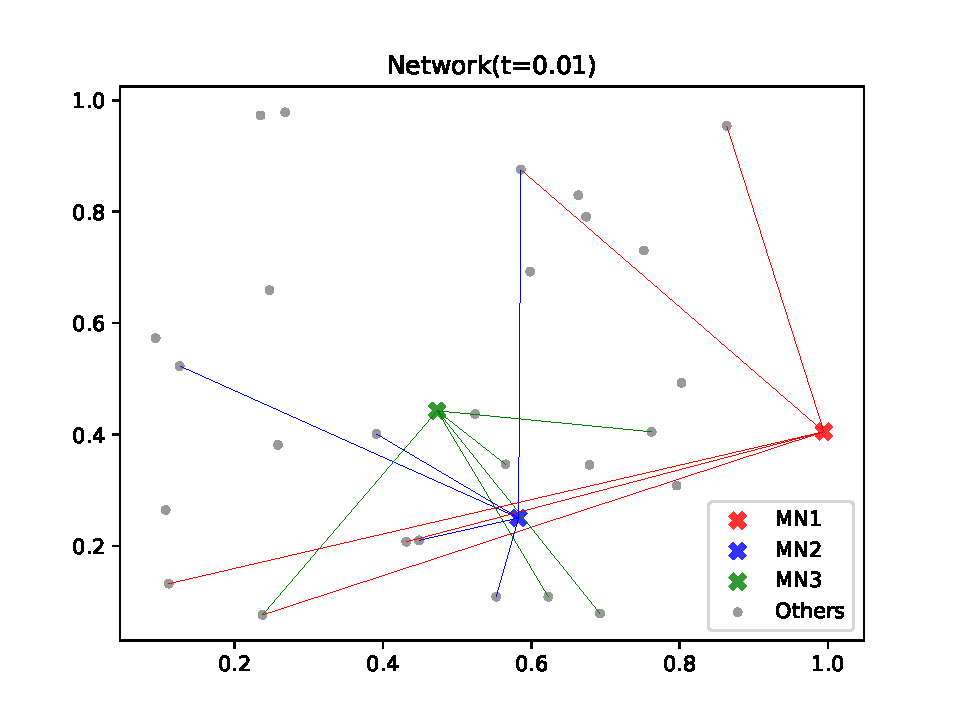
\includegraphics[width = 0.3\textwidth]{Graphs/t_001.pdf}
% 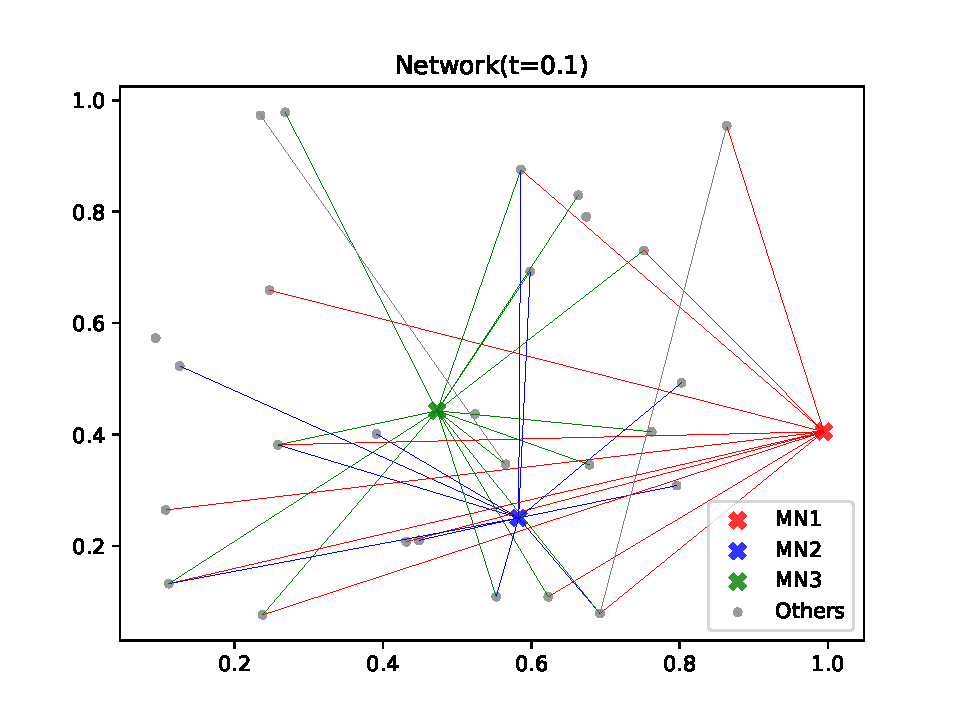
\includegraphics[width = 0.3\textwidth]{Graphs/t_01.pdf}
% 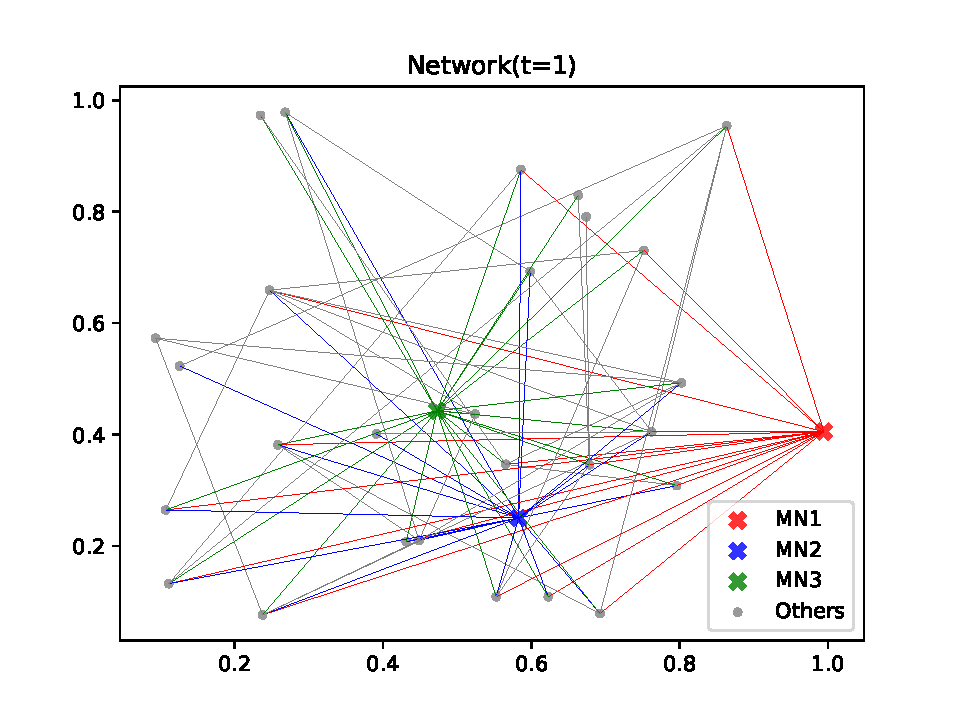
\includegraphics[width = 0.3\textwidth]{Graphs/t_1.pdf}\\
% 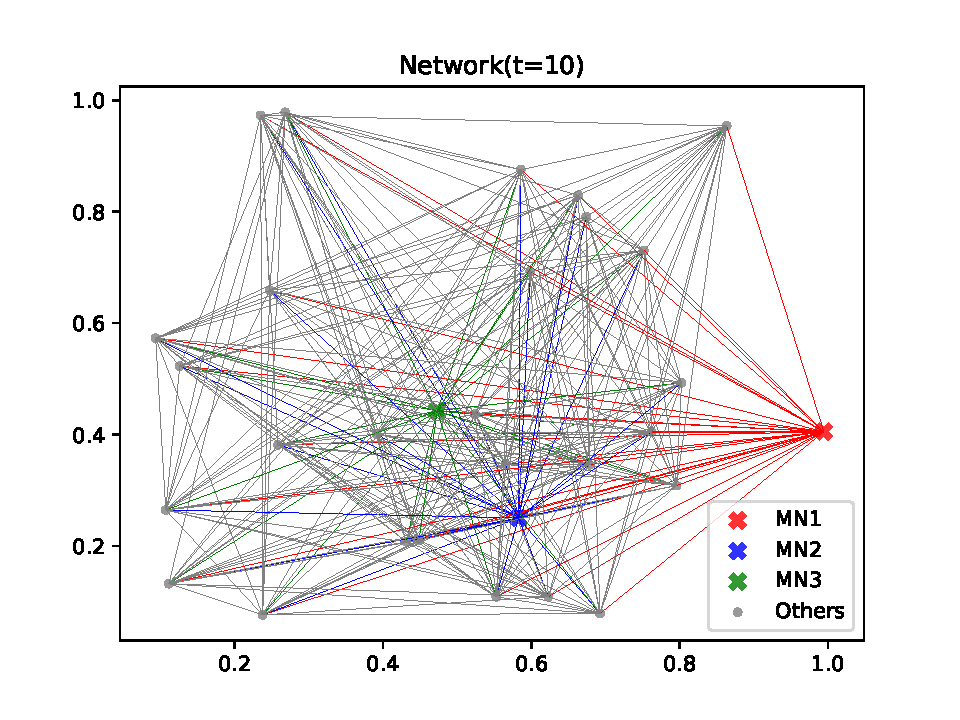
\includegraphics[width = 0.3\textwidth]{Graphs/t_10.pdf}
% 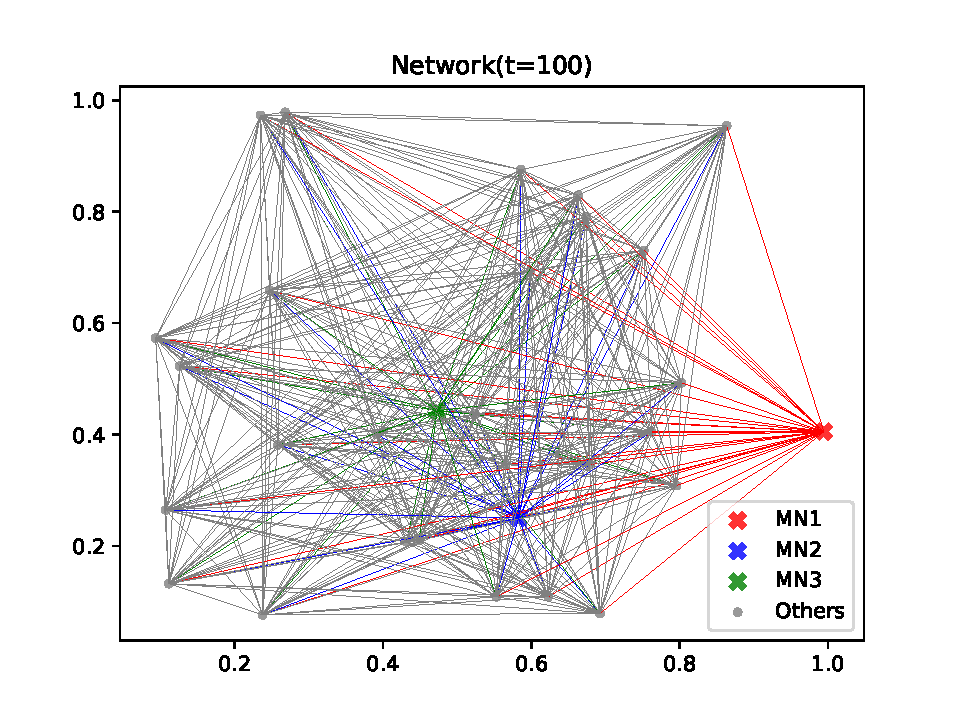
\includegraphics[width = 0.3\textwidth]{Graphs/t_100.pdf}
% \caption{Development of the network with two cell types. The node $n_1$ is represented by ``MN1'' in red. The node $n_2$ is represented by ``MN2'' in blue. The node $n_3$ is represented by ``MN3'' in green. Other nodes are represented by ``Others'' in gray.}
% \label{Fig: development of network}
% \end{figure}






% Footnotes\footnote{This is an example of a footnote.}
% pose no problem\footnote{And another one}.


%!TEX root = Main.tex

\section{Conclusion}

% Analyze the computing complexity. The complexity is mainly caused by the estimation of the (mean) intensity functions, initialization of K-means, and K-means (or the convex relaxation method).

~


%!TEX root = Main.tex

\appendix

\section{Appendix section}\label{app}

TO DO:
\begin{enumerate}
% \item Selection of k.
\item Simulation.
\item Write introduction, and sketch of proof.
\item Re-write model section, clarify assumptions.
\item Basic knowledge about point process (reading).
\item Real data.
% \item Convex relaxation/FPCA (reading).
\end{enumerate}

\subsection{Appendix subsection}

See Appendix \ref{app}.


\section*{Acknowledgements}
See \ref{suppA} for the supplementary material example.


%!TEX root = Main.tex


\begin{supplement}
\sname{Supplement A}\label{suppA}
\stitle{Title of the Supplement A}
\slink[url]{http://www.e-publications.org/ims/support/dowload/imsart-ims.zip}
\sdescription{Dum esset rex in
accubitu suo, nardus mea dedit odorem suavitatis. Quoniam confortavit
seras portarum tuarum, benedixit filiis tuis in te. Qui posuit fines tuos}
\end{supplement}


\bibliographystyle{imsart-nameyear}

\bibliography{/Users/bgemily/Documents/Academic/SC/library}
% \bibliography{/Users/bgemily/Documents/Academic/SC/point\ process}

\end{document}
